\documentclass{article}
\usepackage{amsmath}
\usepackage{mathtools}
\usepackage{enumerate}
\usepackage{hyperref}
\usepackage{dsfont}
\usepackage{bbm}
\usepackage[table]{xcolor}
\usepackage{booktabs}
\usepackage{pgfplotstable}
\usepackage{graphicx}
\begin{document}
\title{Math 480 Final Project}
\author{
  Steiger, Taylor\\
  \texttt{tsteiger@uw.edu}
  \and
  Pak, James\\
  \texttt{jimmypak@uw.edu}
}
\date{Spring 2013}
\maketitle

\newpage
\tableofcontents
\newpage

\section{Preface\label{intro}}
Taylor and James are current undergraduates in the mathematics department at the University of Washington. This paper is their final project for their Math 480 class. Upon reviewing the elements of SAGE dedicated to SVD's, they concluded there was not the functionality included in SAGE necessary to perform rank 1 modifications to the thin SVD. Taylor and James used an article published my Matthew Brand on the mathematics behind rank 1 modifications to the thin SVD titled, "Fast low-rank modifications of the thin singular value decomposition," in order to implement this new funcitonality into SAGE. This paper outlines the steps Brand took and then concludes with a section of the included functionality of SAGE created by Taylor and James.

\section{Introduction\label{intro}}
Matthew Brand created an algorithm to approximate rank-1 additive modifications to the thin SVD. This paper uses Brand's algorithm and published paper to summarize the process and implement it within SAGE. It is important to note that this paper by James and Taylor only uses the first 3 sections of Brand's paper. Brand's paper is referenced at the end of this paper.


\section{SVD\label{svd}}
Consider the real matrix $\mathds{X}{\epsilon}{\mathds{R}^{p\mathrm{x}q}}$.
Then the singular value decomposition (SVD) diagnolizes $\mathds{X}$ with orthonormal matrices $\mathds{U}\epsilon \mathds{R}^{p\mathrm{x}p}$ and $\mathds{V} \epsilon \mathds{R}\label{R}^{q\mathrm{x}q}$.
Then $\mathds{S}=\mathds{U}^T\mathds{X}\mathds{V}$ is diagonal and nonnegative. This is equivalent to saying that it decomposes $\mathds{X}$ into sums of rank-1 matrices from singular value triplets: $\mathds{X} = \mathds{U}\mathrm{diag}{(s)}\mathds{V}^T = \sum_{i} \mathbf{u}_{i} s_{i} \mathbf{v}_{i}^T$ for singluar values of $s_{i}$ on the diagonal of $\mathds{S}$ and singular vectors $\mathbf{u}_{i}$ and $\mathbf{v}_{i}$ taken from the columns of $\mathds{U}$ and $\mathds{V}$.


\section{Additive Modification\label{additive}}
Let $\mathds{A} \epsilon \mathds{R}^{p\mathrm{x}c}$ and $\mathds{B} \epsilon \mathds{R}^{p\mathrm{x}c}$ be arbitrary matrices of rank $c$ and $\mathds{X}{\epsilon}{\mathds{R}^{p\mathrm{x}q}}$ have rank $r$ and economy SVD $\mathds{USV}^T = \mathds{X}$ with $\mathds{S}\epsilon\mathds{R}^{r\mathrm{x}r}$.
Then we are interested in the SVD of the sum:
$$
\mathds{X} + \mathds{AB}^T =
\begin{bmatrix}
\mathds{U} & \mathds{A}
\end{bmatrix}
\begin{bmatrix}
\mathds{S} & 0 \\
0 & \mathds{I}
\end{bmatrix}
\begin{bmatrix}
\mathds{V} & \mathds{B}
\end{bmatrix}^T
$$

Furthermore, let $\mathds{P}$ be the orthogonal basis of the column space of $(\mathds{I}-\mathds{UU}^T)\mathds{A}$ and let $\mathds{R_A}=\mathds{P}^T(\mathds{I}-\mathds{UU}^T)\mathds{A}$.

Then
$$
\begin{bmatrix}
\mathds{U} & \mathds{A}
\end{bmatrix}
=
\begin{bmatrix}
\mathds{U} & \mathds{P}
\end{bmatrix}
\begin{bmatrix}
\mathds{I} & \mathds{U}^T\mathds{A} \\
0 & \mathds{R_A}
\end{bmatrix}
$$.

Let $\mathds{QR_B}=(\mathds{I}-\mathds{VV}^T)\mathds{B}$.

Then
$$
\mathds{X}+\mathds{AB}^T =
\begin{bmatrix}
\mathds{U} & \mathds{P}
\end{bmatrix}
\mathds{K}
\begin{bmatrix}
\mathds{V} & \mathds{Q}
\end{bmatrix}^T
$$

and

$$
\mathds{K}=
\begin{bmatrix}
\mathds{I} & \mathds{U}^T\mathds{A}\\
0 & \mathds{R_A}
\end{bmatrix}
\begin{bmatrix}
\mathds{S} & 0\\
0 & \mathds{I}
\end{bmatrix}
\begin{bmatrix}
\mathds{I} & \mathds{V}^T\mathds{B}\\
0 & \mathds{R_B}
\end{bmatrix}^T
=
\begin{bmatrix}
\mathds{S} & 0\\
0 & 0
\end{bmatrix}
+
\begin{bmatrix}
\mathds{U}^T\mathds{A}\\
\mathds{R_A}
\end{bmatrix}
\begin{bmatrix}
\mathds{V}^T\mathds{B}\\
\mathds{R_B}
\end{bmatrix}^T
$$.

Diagonalizing $\mathds{K}$ as $\mathds{U}'^T\mathds{KV}'=\mathds{S}'$ gives the rotations $\mathds{U}'$ and $\mathds{V}'$ of the extended subspaces
$
\begin{bmatrix}
\mathds{U} & \mathds{P}
\end{bmatrix}
$
and
$
\begin{bmatrix}
\mathds{V} & \mathds{Q}
\end{bmatrix}
$
such that
$$
\mathds{X}+\mathds{AB}^T = \left(
\begin{bmatrix}
\mathds{U} & \mathds{P}
\end{bmatrix}
\mathds{U}' \right)
\mathds{S}'\left(
\begin{bmatrix}
\mathds{V} & \mathds{Q}
\end{bmatrix}
\mathds{V}'\right)^T
$$
is the desired SVD.


\section{Rank-1 Modification\label{rank}}
For the SVD of $\mathds{USV}^T + \mathds{ab}^T$ with vectors $\bf{a}\epsilon\mathds{R}^p$ and $\bf{b}\epsilon\mathds{R}^q$, the equation:

$$
\begin{bmatrix}
\mathds{U} & \mathds{A}
\end{bmatrix}
=
\begin{bmatrix}
\mathds{U} & \mathds{P}
\end{bmatrix}
\begin{bmatrix}
\mathds{I} & \mathds{U}^T\mathds{A} \\
0 & \mathds{R_A}
\end{bmatrix}
$$

can be changed in a partial step by the modified Gram-Schmidt algorithm.
These alterations are expressed as:

$$
\bf{m} \dot{=} \mathds{U}^T \bf{a}; \hspace{1pc}
\bf{p} \dot{=} \bf{a} - \mathds{U}\bf{m}; \hspace{1pc}
\it{R_a} = \|\bf{p}\|; \hspace{1pc}
\mathds{P} = \it{R_a}^{-1} \cdot \bf{p}
$$.

Similarly,

$$
\bf{m} \dot{=} \mathds{V}^T \bf{b}; \hspace{1pc}
\bf{q} \dot{=} \bf{b} - \mathds{V}\bf{n}; \hspace{1pc}
\it{R_b} = \|\bf{q}\|; \hspace{1pc}
\mathds{Q} = \it{R_b}^{-1} \cdot \bf{q}
$$
\bigskip
\\
Expresses the common operations on the last column or on all columns expressed as rank-1 modifications of an SVD $\mathds{USV}^T = \mathds{X}$ to give $\mathds{U}'\mathds{S}'\mathds{V}'^T = \mathds{X} + \bf{ab}^T$\\
\begin{tabular}{ *5l }    \toprule
\emph{Operation} & \emph{Known} & \emph{Desired}& \emph{$\bf{a}$} & \emph{$\bf{b}^T$} \\\midrule
Update    & $\mathds{US}\begin{bmatrix} \mathds{V}^T & 0 \end{bmatrix} = \begin{bmatrix} \mathds{X} & 0 \end{bmatrix}$  & $\mathds{U}'\mathds{S}'\mathds{V}'^T = \begin{bmatrix} \mathds{X} & \bf{c} \end{bmatrix}$& $\bf{c}$  & $\begin{bmatrix} 0, \ldots, 0, 1 \end{bmatrix}$  \\
Downdate & $\mathds{USV}^T = \begin{bmatrix} \mathds{X} & \bf{c} \end{bmatrix}$ & $\mathds{U}'\mathds{S}'\mathds{V}'^T = \mathds{X}$ & \bf{-c} & $\begin{bmatrix} 0, \ldots, 0, 1 \end{bmatrix}$\\
Revise & $\mathds{USV}^T = \begin{bmatrix} \mathds{X} & \bf{c} \end{bmatrix}$ & $\mathds{U}'\mathds{S}'\mathds{V}'^T = \begin{bmatrix} \mathds{X} & \bf{d} \end{bmatrix}$ & \bf{d-c} & $\begin{bmatrix} 0, \ldots, 0, 1 \end{bmatrix}$\\
Recenter & $\mathds{USV}^T= \mathds{X}$ & $\mathds{U}' \mathds{S}' \mathds{V}' ^T = \mathds{X} \left{(} \mathds{I} - \frac{1}{q} \bf{11}^\it{T} \right{)} $ & $ - \frac{1}{q} \mathds{X}\bf{1}$& \bf{1}^T \dot{=}  $\begin{bmatrix} 1, \ldots, 1 \end{bmatrix}$\\\bottomrule
 \hline
\end{tabular}
\bigskip



The equation:
$$
\mathds{K}=
\begin{bmatrix}
\mathds{S} & \bf{0}\\
\bf{0} & 0
\end{bmatrix}
+
\begin{bmatrix}
\bf{m}\\
\|\bf{p}\|
\end{bmatrix}
\begin{bmatrix}
\bf{n}\\
\|\bf{q}\|
\end{bmatrix}^T
$$
gets simplified to a diagonal $+$ rank-1 matrix.
Table 1 shows that specializations of the above equation are the various cases of updating, downdating, and revising individual columns of the SVD.




\section{Reference\label{reference}}
All work within the above sections is taken from Matthew Brand's article on \href{http://www.stat.osu.edu/~dmsl/thinSVDtracking.pdf}{"Fast low-rank modifications of the thin singular value decomposition."}




\section{Implementation in SAGE\label{sage}}


\begin{figure}[ht!]
  \begin{center}
    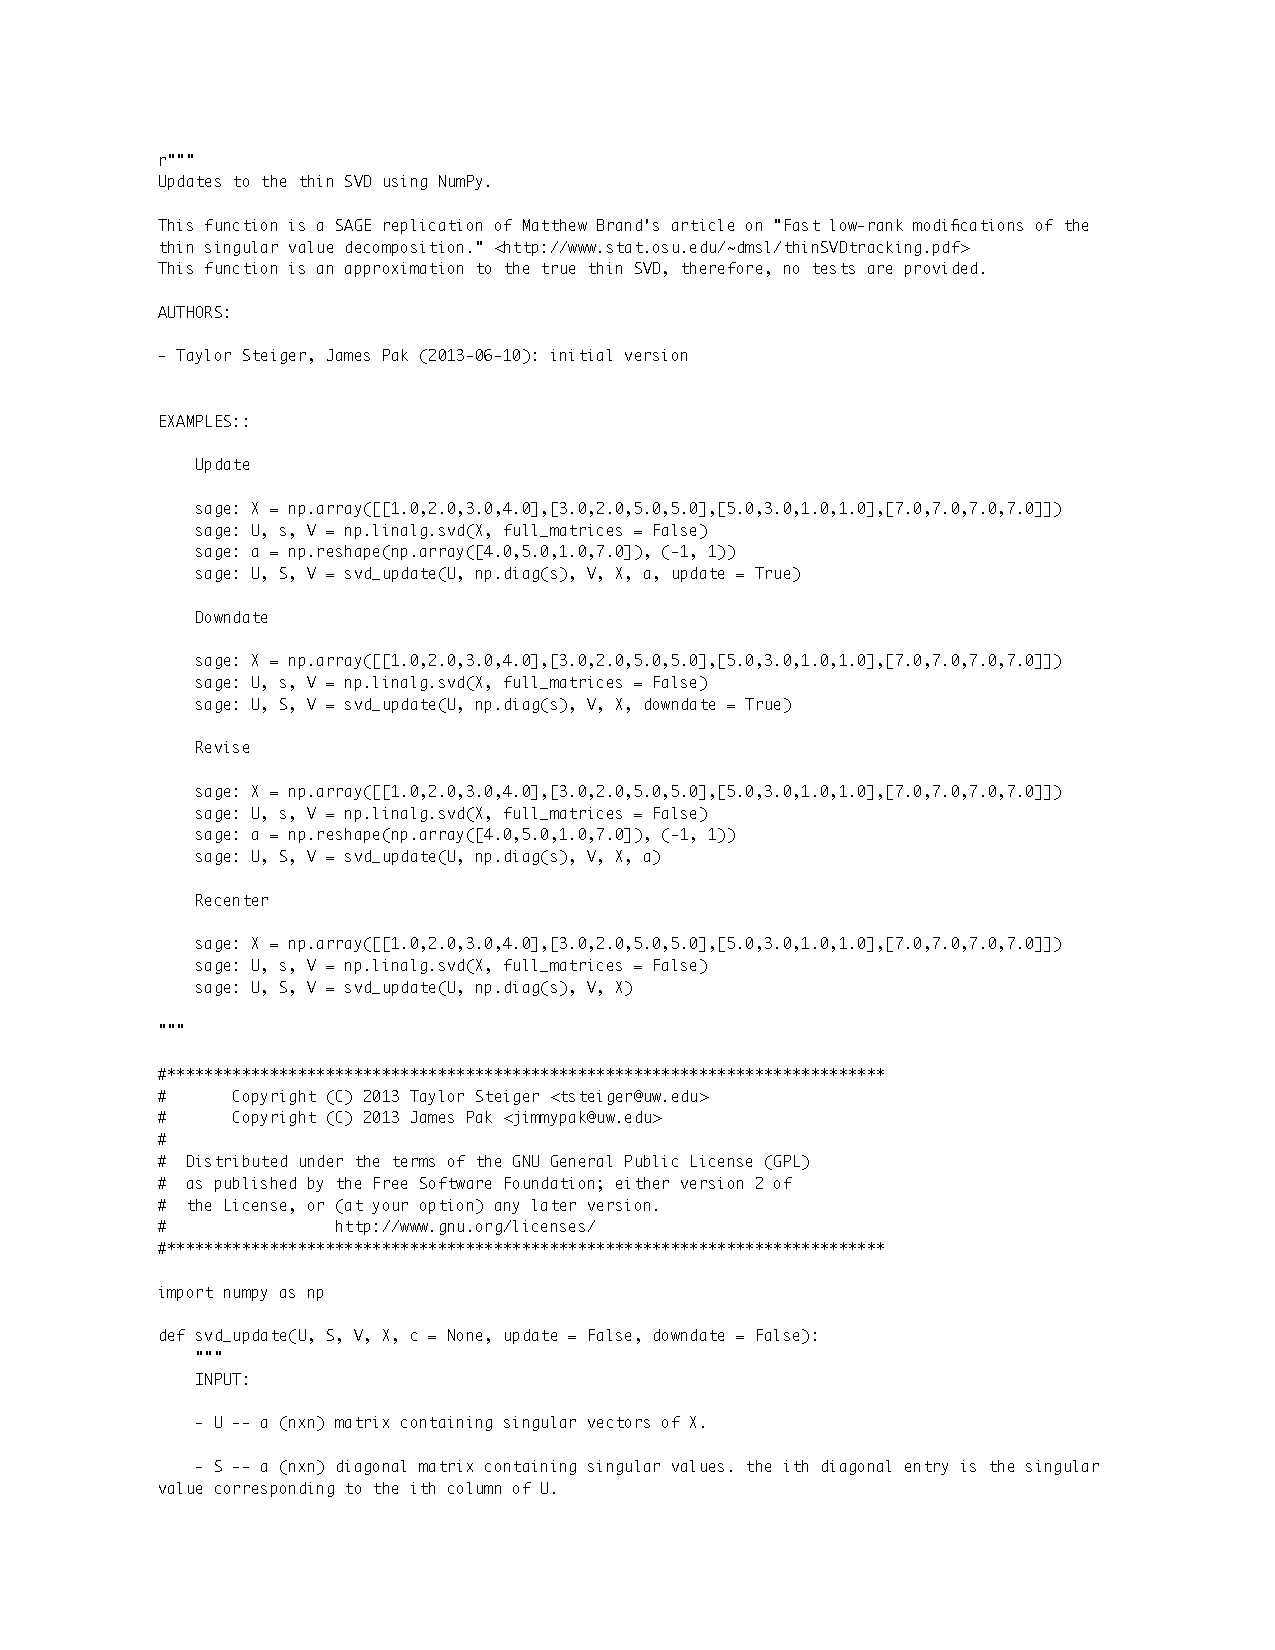
\includegraphics[page=1, bb=0.0in 0.0in 8.5in 10in, scale=.5]{half1.pdf}
    \includegraphics[page=2, bb=0.0in 0.0in 8.5in 9in, scale=.5]{half1.pdf}
    \label{overflow}
  \end{center}
\end{figure}

\begin{figure}[ht1!]
  \begin{center}
    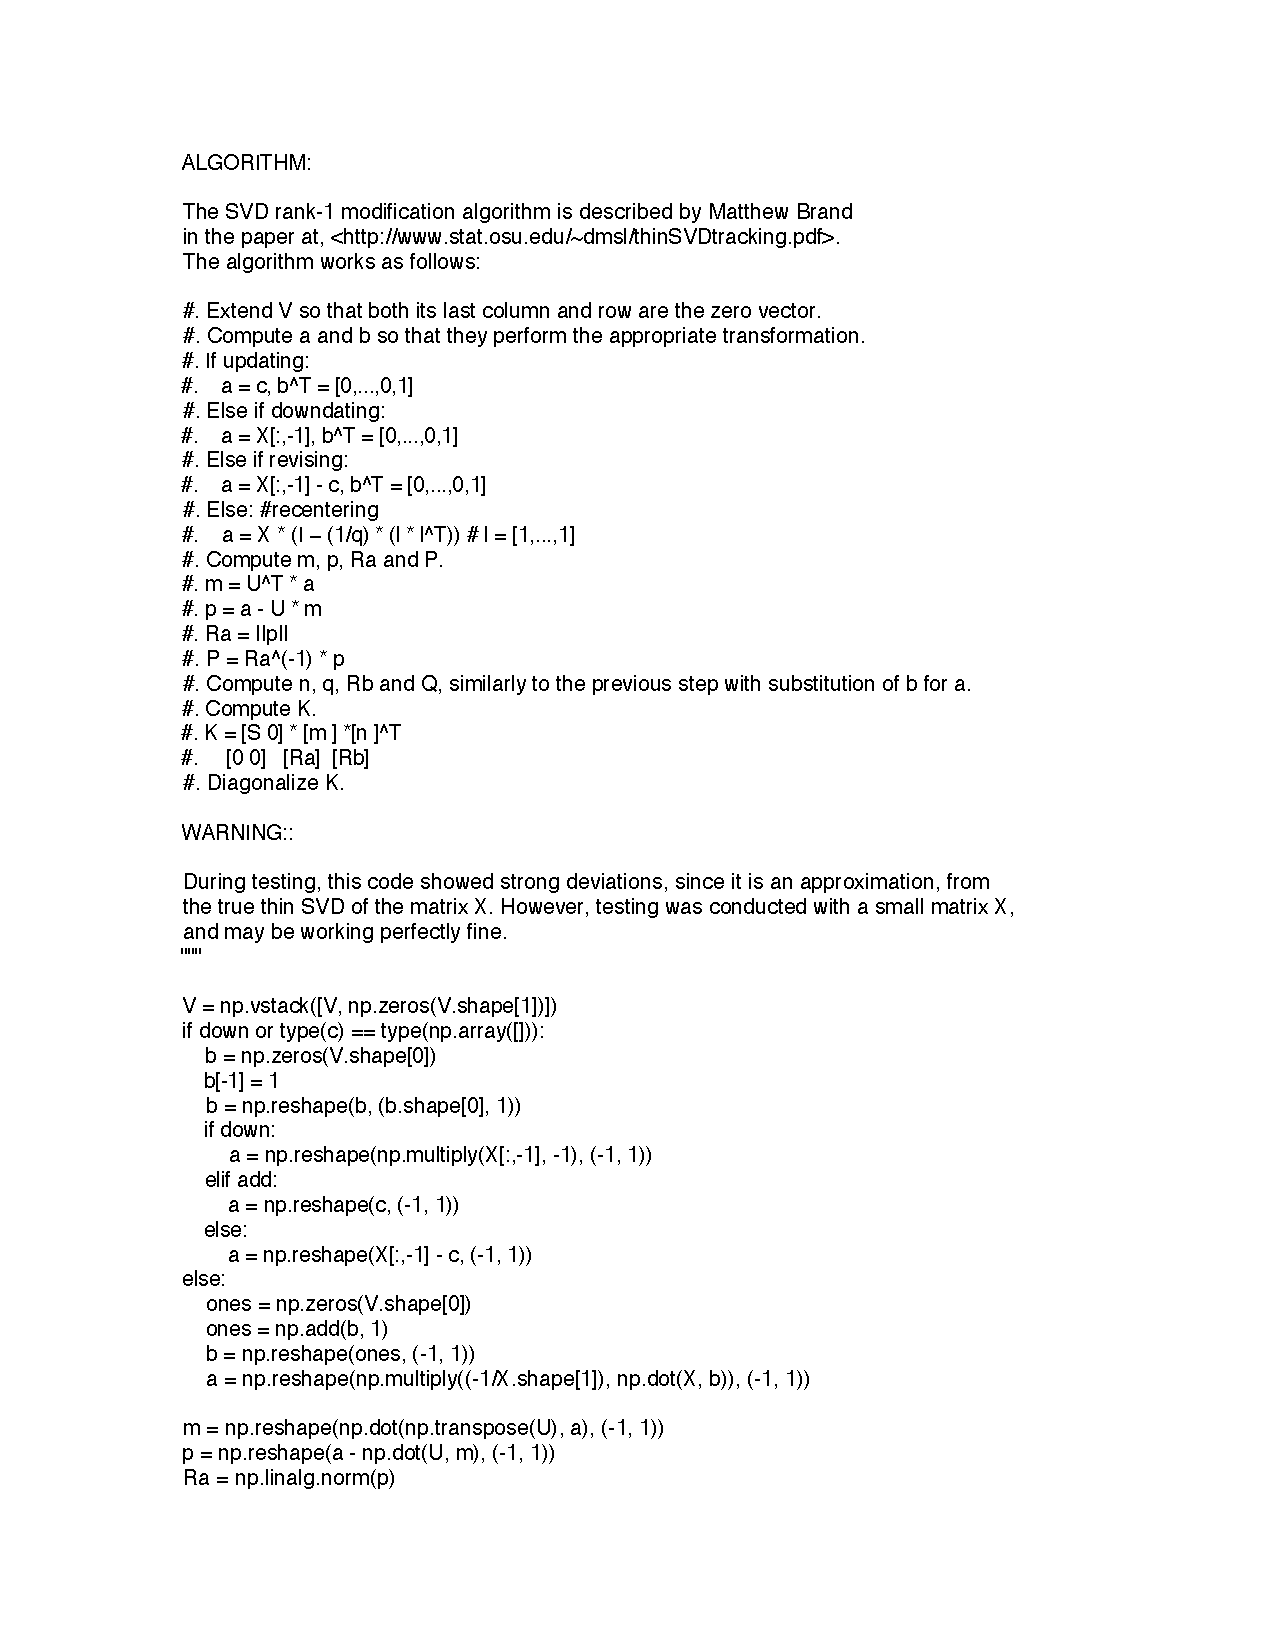
\includegraphics[page=1, bb=0.0in 0.0in 8.5in 10in, scale=.5]{half2.pdf}
    \includegraphics[page=2, bb=0.0in 0.0in 8.5in 9in, scale=.5]{half2.pdf}
    \label{overflow}
  \end{center}
\end{figure}



\end{document}
